\section{Klassediagrammer}
Heisstyringa er delt opp i klasser. Måten vi har implementert dette på er at alle variabler er deklarert static for å holde de internt i en klasse/fil, og innføre set- og getfunksjoner der det trengs. Grunnen til denne oppdelingen er selvfølgelig å få en logisk oppdeling, hvor hver klasse har et veldefinert ansvarsområde. For hver klasse bør det gå greit fram hva de forskjellige variablene og funksjonene gjør, men det er gitt utdypende forklaring ved de mest sentrale.
\subsection{Tilstandsmaskinen}
\begin{figure}
\centering
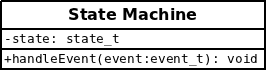
\includegraphics[scale=0.6]{stateMachine.png}
\label{klasse:SM}
\caption{Klassediagram for tilstandsmaskinen}
\end{figure}
Tilstandsmaskinen holder orden på hvilken tilstand heisen står i. 
\begin{description}
\item[handleEvent]\hfill \\
Bestemmer, sammen med tilstandsvariablen, nestetilstand og handling for heisen når den genererer en hendelse.
\end{description}
\subsection{Kontroll}
\begin{figure}
\centering
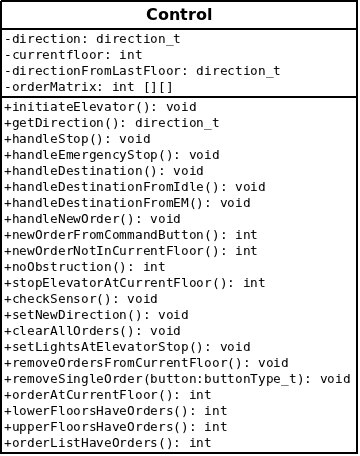
\includegraphics[scale=0.6]{control.png}
\label{klasse:kontroll}
\caption{Klassediagram for kontrollklassen}
\end{figure}
Kontrollklassen inneholder alle funksjoner og variabler som håndterer logikken og den fysiske funksjonen i heisen, som å bestemme retning, at motoren skal startes, hvilke lys som skal tennes, holde orden på bestillingene, og lignende.
\begin{description}
\item[Handlinger]\hfill \\
De forskjellige handlingene (handle$\cdots$) kalles av tilstandsmaskinen, og beskriver den overordnene oppførselen til heisen. Grunnen til tre forskjellige handleDestination-funksjoner er at man i nødstopp- og idletilstand trenger litt annerledes rutiner for å bestemme neste mål for heisen.
\item[Sperre? Vakt?]\hfill \\
newOrderFromCommandButton, newOrderNotInCurrentFloor, noObstruction og stopElevatorAtCurrentFloor er ?sperrer? tilstandsmaskinen bruker for å avgjøre om den skal utføre handlingene.
\item[Checksensor]\hfill \\
En lyttefunksjon som står og går i main-funksjonen for å avgjøre hvilken etasje heisen er i, og gi en handling når den ankommer en etasje.
\item[Heisstyring]\hfill \\
setNewDirection, clearAllOrders, setLightsAtElevatorStop, removeOrdersFromCurrentFloor og removeSingleOrder er funksjoner som påvirker retning, ordre og lys for heisen.
\item[Sammeligning]\hfill \\ 
De fire nederste funksjonene er hjelpefunksjoner som bestemmes av ordrene heisen har. Brukes for å bedre lesbarhet og for å unngå for mye nøsting.
\end{description}
\subsection{User Interface}
\begin{figure}
\centering
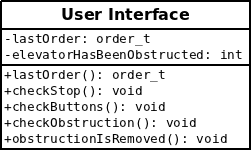
\includegraphics[scale=0.6]{ui.png}
\label{klasse:ui}
\caption{Klassediagram for UI-klassen}
\end{figure}
Denne klassen sørger for å håndtere input fra brukeren, som bestillingsknapper, stoppknapp og obstruksjonsføleren i døra. Den sørger for å sende bestillinger til kontroll.
\begin{description}
\item[Sjekkfunksjoner]\hfill \\
checkButtons, checkStop og checkObstruction løper i main-funksjonen for å for å håndtere input fra brukeren. De genererer også hendelser for tilstandsmaskinen.
\item[LastOrder]\hfill \\
Denne kalles av kontroll-klassen for å returnere siste ordreknapp som ble trykket inn og legge bestilling i ordrelisten.
\end{description}
\subsection{Timer}
\begin{figure}
\centering
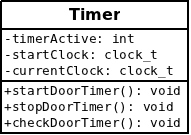
\includegraphics[scale=0.6]{timer.png}
\label{klasse:timer}
\caption{Klassediagram for timeren}
\end{figure}
Timeren er en enkel klasse for å telle ned tre sekunder hver gang døren åpnes i en etasje. Den har to variabler fra time-biblioteket for å telle opp til 3 sekunder, og et heltall som holder orden på om den er aktiv eller iikke.
\begin{description}
\item[checkDoorTimer]\hfill \\
Denne står også og løper i main-funksjonen, og sjekker om nedtellingen er ferdig eller ikke.
\end{description}
\subsection{I/O}
\begin{figure}
\centering
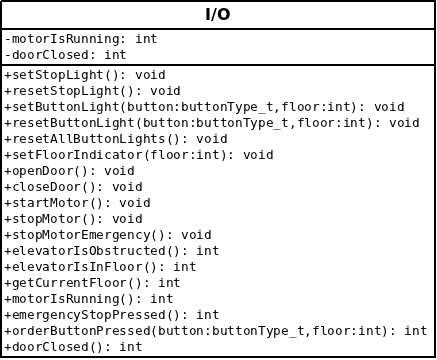
\includegraphics[scale=0.6]{io.png}
\label{fig:class_ui}
\caption{Klassediagram for I/O-klassen}
\end{figure}
I/O klassen er en egenlagt driver for å styre heisen. Dette er vår mest maskinnære klasse, som inneholder funksjoner for alle hardware-relaterte operasjoner som å skru av og på lys, gi signal fra sensoren og sette motorhastigheten. Disse funksjonene implementeres ved hjelp av medfølgende funksjoner i elev.c og io.c
\begin{description}
\item[Lysfunksjoner]\hfill \\
Det er funksjoner for å skru lys av og på. Bestillingslampene kan skrus av en og en, eller alle på en gang som for en nødstopp. Etasjelyset har ingen resetfunksjon, da kun et skal tennes av gangen, og derfor kan det ordnes i setfunksjonen.
\item[Heisaksjoner]\hfill \\
Funksjoner for dør- og motorstyring. Det er egen motorstopp for nødsituasjoner, {\Huge hvorfor?}
\item[Informasjon om Heis]\hfill \\
Funksjoner som registrerer fysisk informasjon om heisen
\item[Knapperegistreringer]
orderButtonPressed blir kalt fra kontroll hver gang man trykker en knapp, og legger etasje og knappetype inn i diagrammet.
\item[vakt? sikring?]\hfill \\
doorClosed er vakt? sikring? som brukes av tilstandsmaskinen.
\end{description}
